% !TeX root = ../thuthesis-example.tex

\chapter{引言}

\section{研究背景与意义}
互联网、物联网、云计算等计算机科学技术经过长时间的共同发展
与不断融合,积累了规模庞大、种类繁多的海量数据,涉及计算机科学、宏观经济、
军事科技、医疗卫生等诸多领域\cite{2022968}。截至2012年,
技术上可在合理时间内分析处理的数据集大小单位为艾字节(EB)
\cite{DBLP:journals/jbd/TsaiLCV15}。
在这些海量数据之中,有一类按照数据生成的时间顺序,把同一个变量或
记录的数据值,或者高维数据的一个元组,排列而成的记录数据信息,
被称为时间序列。时间序列是工业界应用广泛的、与时间维度相关的
高维数据,也是数据挖掘技术的一种主要研究对象。

大多数时间序列中的观测量会随着时间的推移生成有价值的规律
\cite{DBLP:conf/sdm/MueenKZCW09},
其中某些规律在同一个时间序列中多次重复出现,这类规律称为模式。
时间序列中蕴含着多种多样的模式,挖掘出时间序列中蕴含的模式,
既可以为未来的决策提供理论与数据支持,又可以检测、判断、预防突发
错误的出现,指导实际生产。因此,时间序列模式挖掘是时间序列分析和
数据挖掘中的重要组成部分。在多样化的模式中,对称模式因为具有独特的
物理意义,在多种应用场景的时间序列数据中大量出现,具有重要的
研究价值\cite{2022968}。然而,由于时间序列数据的特殊性,对称模式的挖掘也
存在许多困难。

时间序列对称模式包括两种类别,一种是具有全局对称性的时间序列,
称之为全局对称模式。另一种是时间序列中包含的具有对称性的子序列集合,
即分段对称模式。对于全局对称时间序列来说,
从数学角度判断其对称性的方式十分简单,确定对称中心,
并计算中心一侧序列是否为另一侧的镜像即可。图~\ref{fig:symmetric_string}
展示了对称字符串序列示意图,该序列在“D”两侧的子串互为镜像,
则为对称(回文)字符串序列\cite{DBLP:journals/corr/abs-2003-08211}。
然而,时间序列的对称性并不像回文字符串序列
的对称性具有非常严格的数学定义,并不存在严格统一的对称中心。
图~\ref{fig:no_symmetic_center}展示了血压测量中力感测电阻器(FSR)
信号的变化示意图,尽管在物理意义上一次心跳过程的压缩和舒张阶段时间序列
具有对称性。然而,由于压缩阶段和舒张阶段的时长不一致,
采集点的个数不同,其对称中心并不严格位于时间的中点。
因此,在计算序列对称性时,不能简单地查找对称中心并根据对称中心将时间序列
分段,以免计算的对称度不准确\cite{DBLP:journals/csda/DaiNG18}。
除此之外,由于物理设备、数据采集和数据传输
中遇到的问题,实际应用场景中的时间序列可能不是等间隔采样的,导致不同阶段
的数据点密度不一致,这种情况同样会造成对称中心点的不确定性。
\begin{figure}
  \centering
  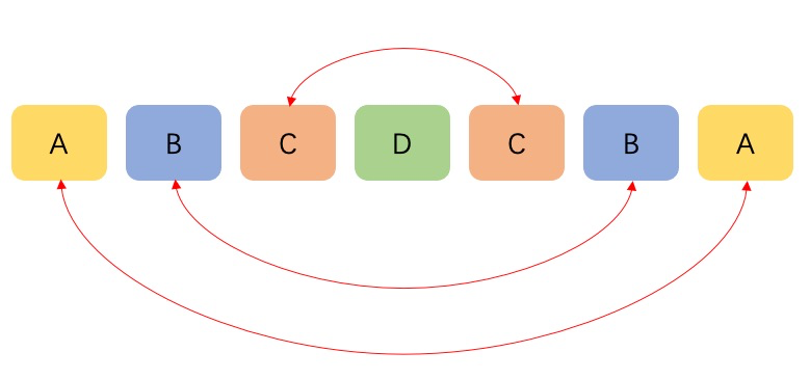
\includegraphics[width=0.76\linewidth]{symmetric_string.png}
  \caption{对称字符串序列}
  \label{fig:symmetric_string}
\end{figure}

\begin{figure}
  \centering
  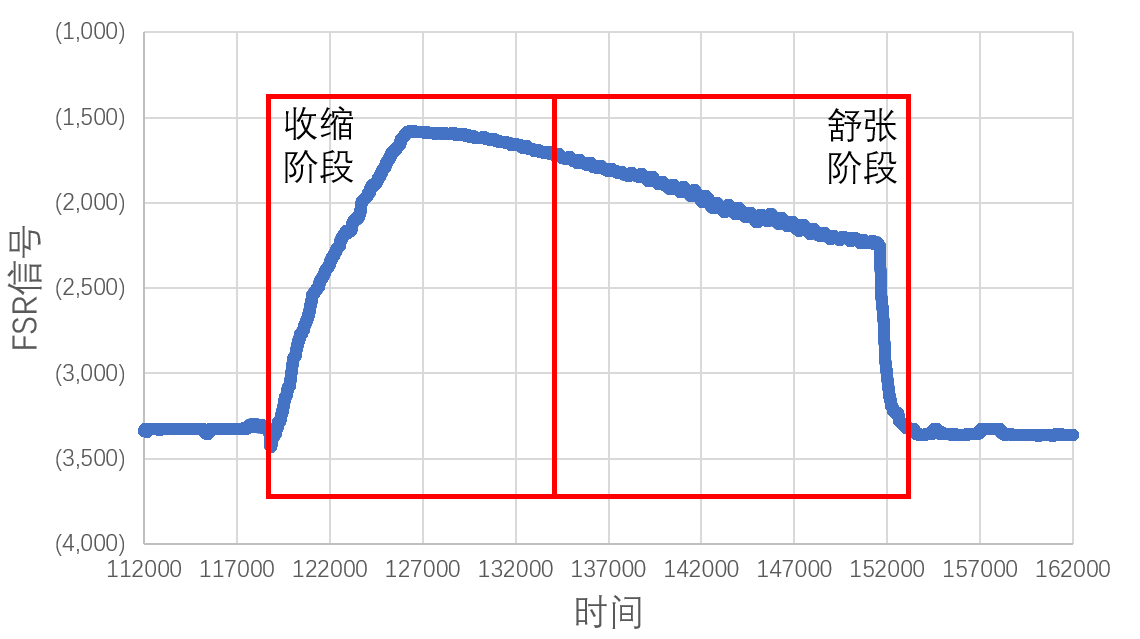
\includegraphics[width=0.76\linewidth]{no_symmetic_center.png}
  \caption{对称时间序列反映无严格对称中心的案例}
  \label{fig:no_symmetic_center}
\end{figure}

此外,由于采样频率不同以及数据随机性较大,时间序列在对称性匹配过程中
不可避免地存在一些失配现象\cite{DBLP:journals/corr/abs-2202-05403}。
图~\ref{fig:mismatch}展示了某辆挖掘机
在作业过程中动臂提升工况的变化示意图,该序列为一次挖掘作业的动臂提升工况
时间序列,具有物理上的对称性。然而,由于抬臂阶段产生了红框所示的数据采集
缺失,导致动臂提升工况时间序列的抬臂和降臂阶段并不完全匹配。因此,
在对称模式的挖掘过程中,需要考虑到因为部分失配导致的对称度计算结果偏差问题。

除了利用对称中点截断时间序列计算对称性之外,使用原始时间序列和
其反转时间序列\cite{DBLP:journals/entropy/ChvostekovaJK21}
的相似性来度量对称性也是一种常见的方法。然而,
时间序列的对称性与时间间隔、序列模式和数据特征密切相关。在实际工业场景中,
原始和反转时间序列在时间线上不对齐的情况时有发生,不存在严格的一一对应关系,
使用传统的匹配方法,无法进行全局匹配度量。图~\ref{fig:time_series_align}
对比了某辆运煤车在行驶过程中生成的纬度时间序列不同的匹配方式,
可以看出,一一对应的匹配方式存在大量的未对齐点,
由此计算得到的对称度明显偏大。而全局匹配方式则应该从全局匹配
角度为原始和反转时间序列上的每对点求得最佳匹配,
从而使计算得到的对称度最高。因此,需要立足于时间序列的时间和
全局数据特征挖掘时间序列的对称性。
\begin{figure}
  \centering
  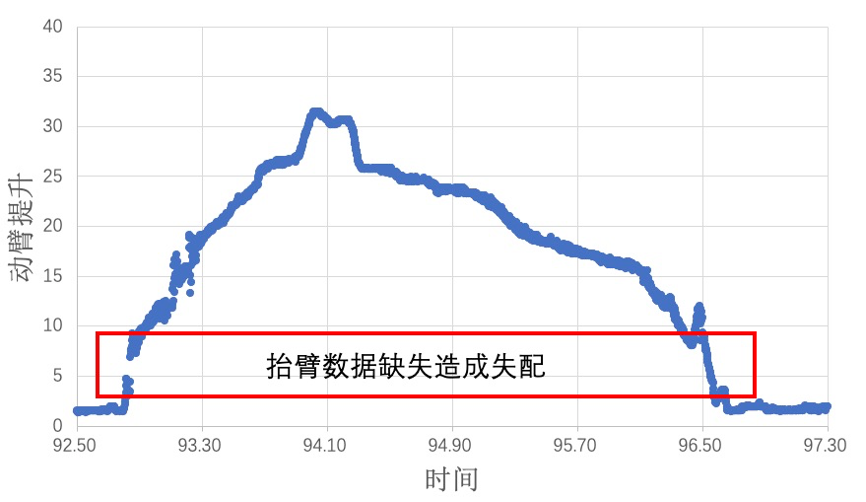
\includegraphics[width=0.76\linewidth]{mismatch.png}
  \caption{对称时间序列反映随机失配现象的案例}
  \label{fig:mismatch}
\end{figure}
\begin{figure}
  \centering
  \subcaptionbox{一一对应\label{fig:time_series_align-a}}
    {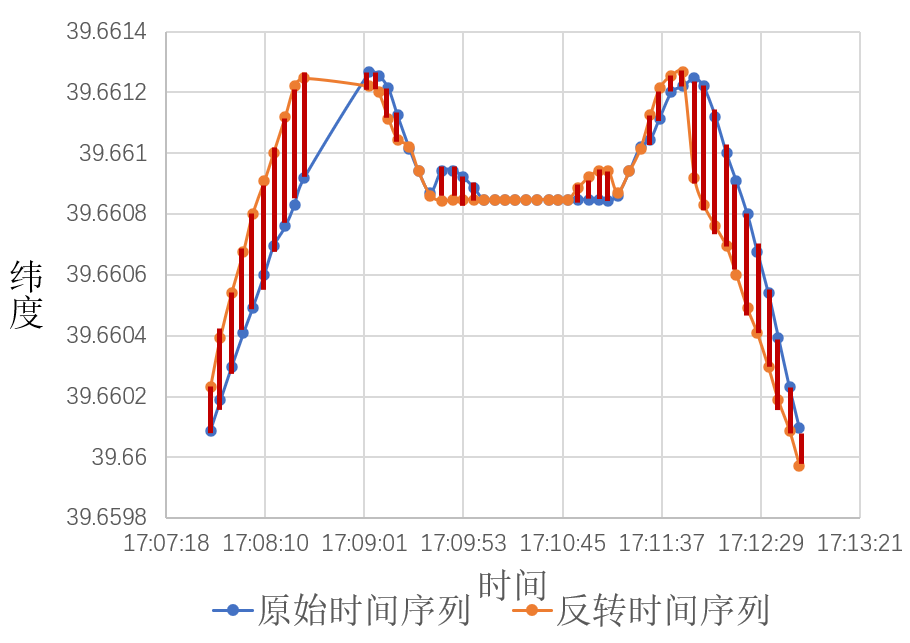
\includegraphics[width=0.49\linewidth]{time_series_align-a.png}}
  \subcaptionbox{全局匹配\label{fig:time_series_align-b}}
    {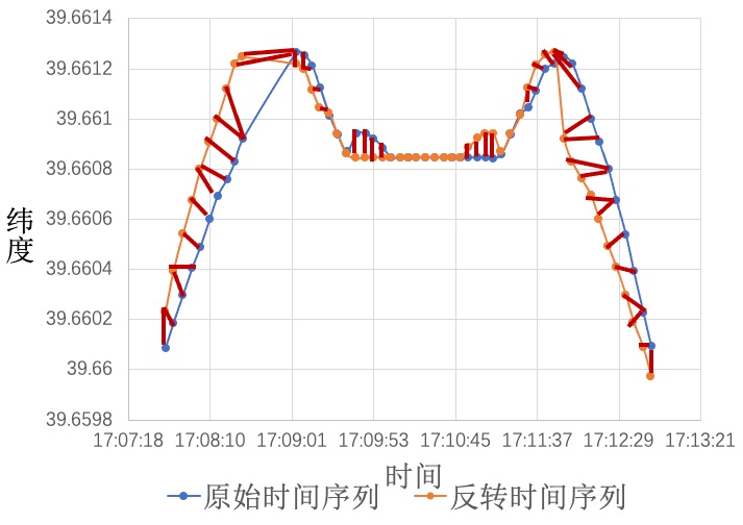
\includegraphics[width=0.49\linewidth]{time_series_align-b.png}}
  \caption{对称时间序列反映不对齐现象的案例}
  \label{fig:time_series_align}
\end{figure}

全局时间序列对称模式的挖掘需要立足于时间序列的整体数据特征。
然而,时间序列中可能蕴含着具有对称性的子模式。
图~\ref{fig:segement_symmetric_pattern}展示了在挖掘机
作业过程中斗杆外摆工况变化形成的时间序列。在该案例中,
多种对称子模式聚合在一条长时间序列之中,
由于传感器采样和数据传输的问题,存在包括
缺失点、异常点、噪声点等诸多问题\cite{DBLP:conf/sigmod/SongZWY15},
这些问题都会干扰对称模式挖掘算法的效果。
并且,挖掘对称子模式需要设定子模式的长度以对长时间序列进行分段
\cite{DBLP:journals/tist/MuralidharTCCRP20},
在给定时间序列的长度约束的前提下,挖掘出的对称子序列可能存在重叠情况,
从而导致后续数据分析和统计存在误差。
\begin{figure}
  \centering
  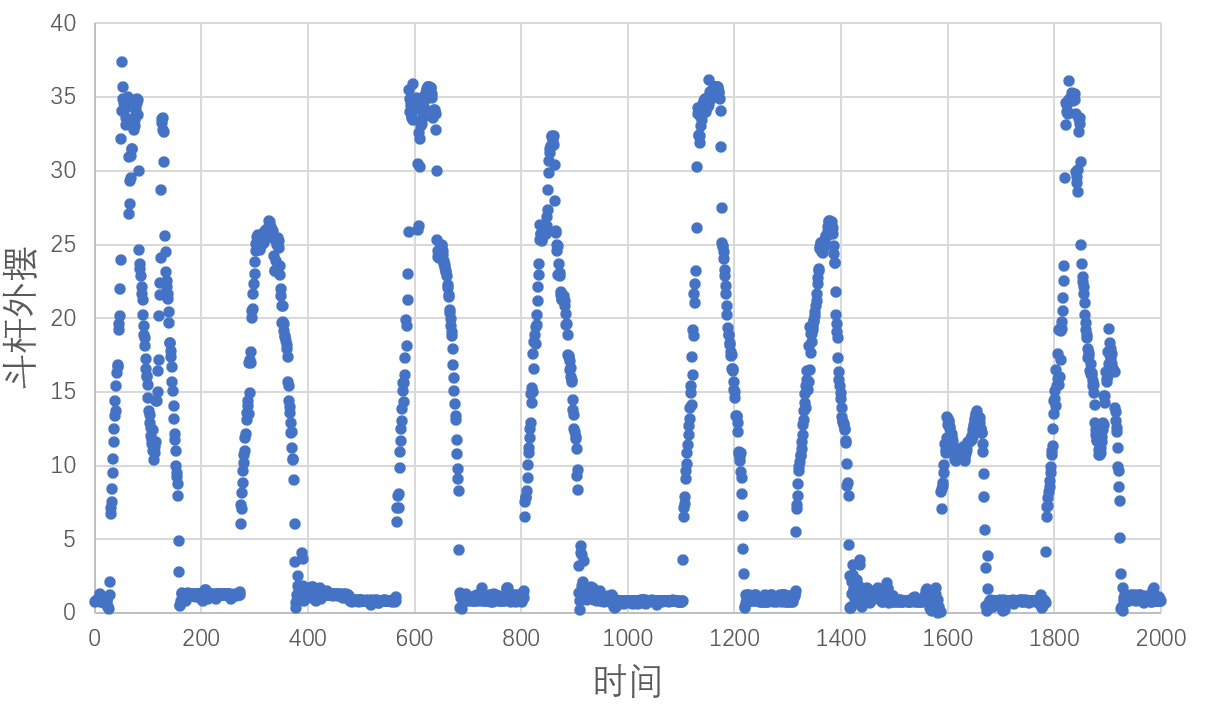
\includegraphics[width=0.76\linewidth]{global_symmetry.png}
  \caption{分段挖掘时间序列对称子模式的案例}
  \label{fig:segement_symmetric_pattern}
\end{figure}

总之,时间序列中的对称模式往往具有某种具体的物理意义,挖掘
对称模式对于轨迹跟踪,作业分析,异常检测和序列预测都具有重要价值。
然而,时间序列的复杂性和不确定性为对称模式挖掘带来了诸多挑战。
基于此,本文提出了一类准确高效的时间序列对称模式挖掘算法,
并将该算法扩展到了流式数据场景,之后经过实验验证了算法的
效果和性能,最后基于Apache IoTDB\cite{10.14778/3415478.3415504}的
存储特点设计了基于UDF和元数据的两种实现,
为用户在不同应用中的模式挖掘提供选择。


\section{研究内容与贡献}
为解决上述问题,本文将研究一类精确高效的时间序列对称模式挖掘方法,具体包含
以下四个方面:
\begin{enumerate}
  \item 全局时间序列的对称性并没有标准的度量方法,现有的基于对称中心与
  原始和反转时间序列的方法都存在问题。不同于回文字符串,时间序列并
  不存在严格统一的对称中心,通过对称中心截取子序列度量对称性的方法
  其效果极不稳定。直接通过原始时间序列和其反转时间序列的相似性度量
  对称性的方法可以避免确定对称中心的问题,但是重复计算,时间不对齐等
  问题也会导致对称性度量结果偏大,从而影响对称模式挖掘结果的准确性。
  因此,如何定义一种准确高效的时间序列对称性度量方法成了首要的目标。
  \item 在分段时间序列上挖掘对称子模式是一个多步骤的算法框架,
  不仅需要度量子序列的对称性,而且,对称时间子序列并不要求原始时间序列
  和其反转时间序列完全相同,只需要两者的距离在指定阈值范围内即可。
  因此,本文需要通过计算阈值来挖掘出真正的对称子序列。此外,时间序列中
  蕴含的对称模式可能存在重叠,需要设计算法过滤重叠的对称子序列,
  从而挖掘出不重叠的对称子序列集合,即分段对称模式。
  \item 对于流数据上的对称模式挖掘,
  由于无法预知时间序列的全貌,
  静态的对称性度量算法失效。
  流数据随时间顺序到达且只有一次处理机会,因此,
  流式算法要在每个新数据点到来时就完成计算,
  并尽量快速高效地进行响应,
  这要求重新设计流式的对称模式挖掘算法。
  \item Apache IoTDB是一个面向时间序列的原生数据库,
  提供了基于UDF接口和元数据的数据分析扩展功能。
  其中,基于UDF的实现不会影响写入性能而在每次查询时重新计算
  \cite{DBLP:journals/jiis/Castro-LopezBL20},
  而基于元数据的实现则会在写入时保存信息以在查询时加速性能
  \cite{DBLP:phd/hal/Zhang19c}。
  两种方式分别适用于读写负载不同的应用场景,本文需要结合这两种
  方式提供对称模式挖掘算法的不同实现,为用户数据分析提供更多选择。
  
\end{enumerate}

基于以上的研究内容,本文主要贡献如下:
\begin{enumerate}
\item 定义了对称模式和全局时间序列对称性度量算法。
本文所挖掘的对称模式是关于中心点前后对称的时间序列模式,
其对称性由自定义的全局对称性度量算法进行计算,再根据时间序列
相邻点的距离特征作为阈值过滤对称时间序列作为全局对称模式。对称模式
在实际工业生产中非常常见,具有很高的应用价值。
\item 提出了分段时间序列对称模式的挖掘方法,并给出了具体的算法。
设定对称子序列的长度约束,采用分段对称性度量算法计算出时间子序列的对称度,
然后使用由时间序列数据特征和对称度分布特征确定的对称度阈值
分类得到对称子序列,最后根据获取数量最多对称子序列的贪心策略,
计算得到所有不重叠的分段对称模式。
\item 扩展了时间序列对称模式挖掘算法的应用,
提高了算法的执行效率。
针对流式数据实时到达的特征优化了对称模式挖掘的状态方程,
每生成一个新的数据点,实时计算出以当前数据点为终点的
子序列对称性,根据对称性阈值即时筛选出对称模式。
\item 本文采用了来自UCR\cite{DBLP:journals/ieeejas/DauBKYZGRK19}
和真实工业场景中的时间序列数据集在
挖掘对称模式的F值,准确率以及时间开销方面进行了实验,
并与多种现有相关方法进行了对比。
结果表明:本文所提出的时间序列对称模式挖掘算法在
挖掘效果方面表现最优,同时在时间开销方面有着几乎最佳的性能。
此外,本文针对IoTDB系统实现了基于UDF和元数据的
两种不同的对称模式挖掘算法实现,并把它们集成到
数据质量分析工具IoTDB-Quality中。一方面,
完善了IoTDB在时间序列模式挖掘上的功能。
另一方面,通过挖掘对称模式,
用户可以继续对时间序列进行数据分析,
进一步推动了IoTDB系统的应用。
\end{enumerate}

\section{论文组织结构}

本文包括7个章节,每章介绍的具体内容如下所示:

第 1 章为引言部分,主要介绍了时间序列的数据特点和
对称模式挖掘的挑战,在此基础上指出了全局和分段对称模式
挖掘的研究内容,并分析了两种算法在理论和应用上的贡献。

第 2 章对本文所用的时间序列、对称模式等基本概念进行了定义,
之后介绍并对比了国内外在序列相似性度量和模式挖掘上的研究。

第 3 章提出时间序列全局对称模式挖掘算法,
本算法利用区间动态规划和最优匹配的算法思想计算对称度,
再根据时间序列数据特征确定全局对称度阈值,从而挖掘出全局对称模式。
之后,本章在流式数据上对全局对称模式挖掘算法进行了扩展,
通过优化对称度状态使得在新增数据点到来时能以$O(n)$的
时空复杂度挖掘全局对称模式,在实现中有重要的应用价值。

% 通过实验验证,本算法在对称模式挖掘效果和时间效率上都高于现有
% 其他算法。

第 4 章提出时间序列分段对称模式挖掘算法。
本算法利用分段对称性度量算法计算出时间子序列的对称度,
再根据时间序列数据特征和对称度分布特征确定分段对称度阈值,
通过阈值分类得到对称子序列之后
再利用贪心策略过滤重叠进而挖掘出分段对称模式。
此外,本章还对基于元数据的分段对称模式挖掘算法实现细节
进行了介绍,在一写多读的查询场景提高了分段算法的查询分析性能。
% 对时间序列对称模式的挖掘进行了扩展。
% 本文首先介绍了流式时间序列对称模式挖掘的难点,
% 并对此扩展了对称模式挖掘的状态方程,
% 提高了流式对称模式挖掘的效率。
% 此外,本文还根据对称模式长度不一的问题,
% 提出了可伸缩的自适应窗口挖掘更加完整的对称时间序列。
% 最后通过实验验证了本算法在流式数据上能保证极高的对称性度量性能,
% 且挖掘出的对称模式具有较高的完整性。

第 5 章对时间序列对称模式挖掘算法进行实验验证和结果分析。
首先,本文在UCR中选择了4个数据集,从多个维度将全局
对称模式挖掘算法与基于对称中心和原始反转时间序列相似性的算法
进行对比。然后,本文设计了1个合成数据集和3个真实数据集,
对分段对称模式挖掘算法进行效果和性能验证。并且,
在真实工业数据集上对基于UDF和元数据的分段算法的写入和查询性能
进行对比实验,证明了不同实现方式在不同应用场景中的适应性。

第 6 章介绍了对称模式挖掘方法的系统实现。
首先介绍了IoTDB为用户提供的查询分析功能扩展框架,
基于此框架分别实现了全局和分段对称模式挖掘算法,
其中,对分段算法提供了基于UDF和元数据的External UDF和
Built-in UDF两种实现。最后在IoTDB Client和Apache Zepplin
\cite{DBLP:conf/xsede/ChengLJXC18}
展示了对称模式挖掘算法的结果。

第 7 章对本文的工作进行分析总结,并指出了未来工作的主要方向。 
